\documentclass[11pt]{article}

\usepackage[margin=1in]{geometry}
\usepackage{booktabs}
\usepackage{graphicx}
\usepackage{hyperref}
\usepackage[numbers,sort&compress]{natbib}
\usepackage{microtype}
\usepackage{amsmath}
\usepackage{enumitem}

\title{MeTTa-Scaffolded Repair Curricula for TRM-Infused Hermes Skills\\
\large Provisional Addendum and Data Campaign Plan}
\author{Hermes Skills Research}
\date{April 26, 2026}

\begin{document}
\maketitle

\begin{abstract}
This addendum describes a methodology for improving TRM-infused Hermes skills using MeTTa-style symbolic scaffolds as a data-curation and control-plane layer. The central observation is that many benchmark failures are not opaque failures of latent reasoning; they are semi-failed outputs with typed, verifier-visible defects. We therefore construct a near-miss repair curriculum that turns those outputs into repair, verifier, and commit/veto training rows. A local Qwen2.5-3B Q4 benchmark suggests that retrieved repair-training context improves commit/veto decisions, but does not yet solve repair-action selection. We treat this as a provisional scale-floor result and defer the full paper claim until matched 9B and 27B benchmarks are run.
\end{abstract}

\section{Motivation}

Hierarchical and recursive reasoning models have reopened the question of whether compact specialized models can perform useful reasoning work without relying on very large language models for every step. HRM proposes a two-timescale recurrent architecture with strong sample efficiency on puzzle-like reasoning tasks \citep{wang2025hrm}; TRM simplifies this direction into a small recursive network with strong ARC-style generalization claims \citep{jolicoeurmartineau2025trm}. In parallel, MeTTa and OpenCog Hyperon provide a reflective metagraph programming substrate for representing rules, programs, and cognitive procedures as rewriteable symbolic objects \citep{goertzel2021metta,meredith2023metametta}.

Our Hermes setting combines these threads with instruction-tuned tool-use models such as Hermes 3 \citep{teknium2024hermes3} and Prime Intellect-style verifier environments for large-scale RL and evaluation \citep{primeintellect2025intellect3}. The specific research question is narrower than broad AGI: can MeTTa-scaffolded symbolic state make TRM training and deployment more data efficient for skill components such as repair, validation, routing, and commit control?

\section{Method}

We convert benchmark traces into a near-miss repair curriculum. Each row records the environment family, TRM role, failed or semi-failed candidate, verifier label, proposed repair action, and target commit decision. This makes a failed output trainable in multiple ways: as a verifier example, a repair example, a positive preservation example, or a hard negative for a commit/veto gate.

The current split is leakage-aware. Policy variants for the same base case remain in the same split, and rare failure labels are reserved for unseen-family holdout. Figure~\ref{fig:splits} summarizes the resulting data shape. The split is a training artifact, not itself a benchmark claim.

\begin{figure}[t]
  \centering
  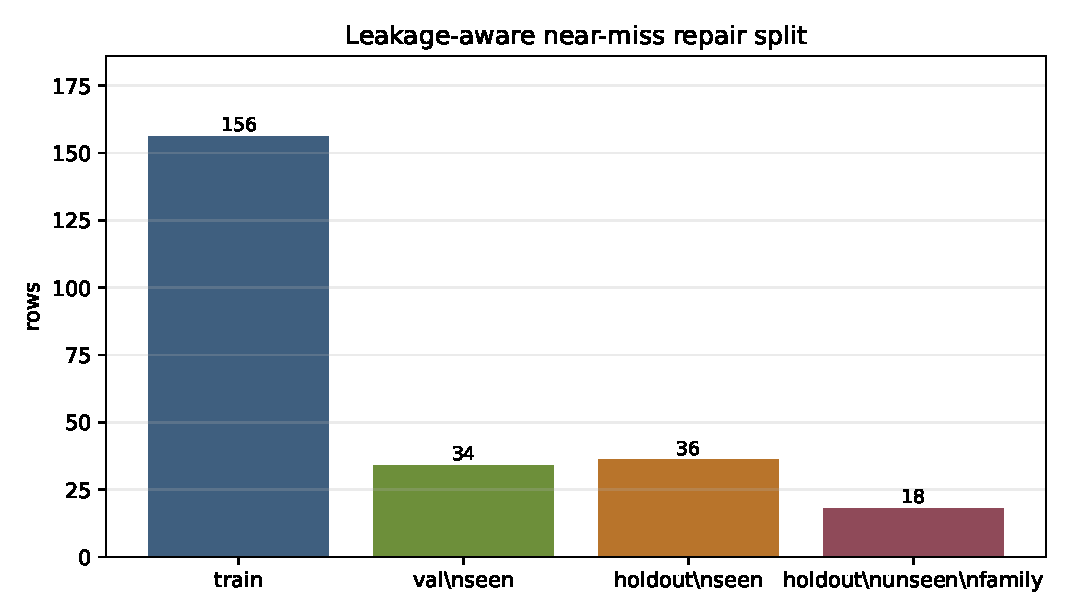
\includegraphics[width=0.82\linewidth]{figures/fig_split_counts.pdf}
  \caption{Near-miss repair curriculum split. The train split supplies repair/verifier/commit rows; seen and unseen holdouts separate case-level generalization from failure-family transfer.}
  \label{fig:splits}
\end{figure}

\begin{table}[t]
  \centering
  \begin{tabular}{lrrrr}
    \toprule
    Split & Rows & Exact positive & Repair success & No-gain / hard negative \\
    \midrule
    Train & 156 & 46 & 58 & 40 \\
    Validation, seen family & 34 & 14 & 12 & 6 \\
    Holdout, seen family & 36 & 8 & 12 & 10 \\
    Holdout, unseen family & 18 & 3 & 9 & 6 \\
    \bottomrule
  \end{tabular}
  \caption{Leakage-aware split counts from the current near-miss repair curriculum. Partial repair improvements account for the remaining rows in each split.}
  \label{tab:splits}
\end{table}

\section{Local 3B Rudder Benchmark}

Before training new TRM weights, we tested whether a small local model can act as a control-plane rudder over the generated Pure-TRM rows. The benchmark uses all 88 non-train rows and compares two arms:

\begin{itemize}[leftmargin=*]
  \item \textbf{raw\_3b\_rudder}: the model sees only the eval state and chooses a repair action plus \texttt{commit} or \texttt{reject\_or\_abstain};
  \item \textbf{repair\_training\_rudder}: the model sees the same eval state plus four retrieved training examples from the near-miss curriculum.
\end{itemize}

The prompt intentionally omits the target repair gate and target bucket from eval state. This makes the result a pre-training control-plane benchmark rather than a replay of labels.

\begin{figure}[t]
  \centering
  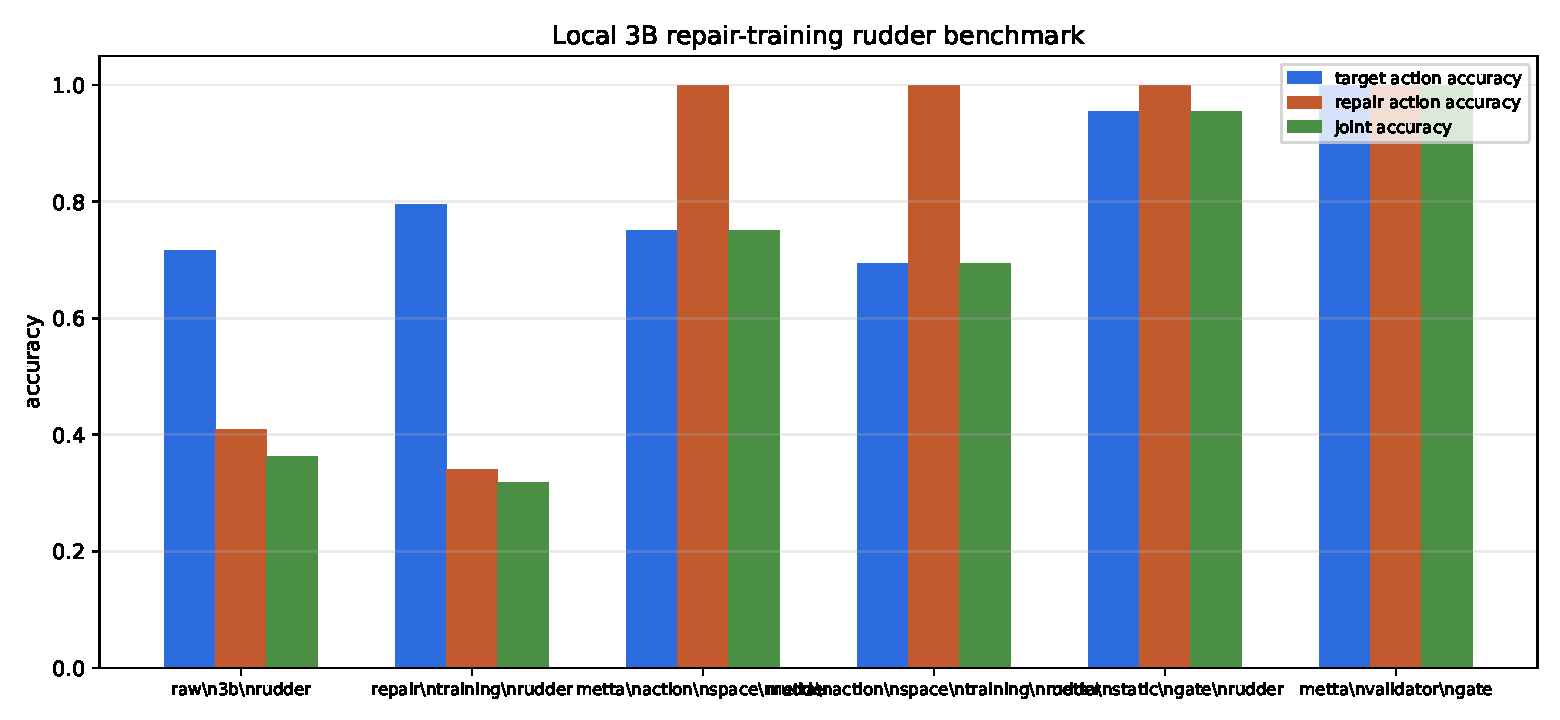
\includegraphics[width=0.86\linewidth]{figures/fig_rudder_summary.pdf}
  \caption{Local Qwen2.5-3B Q4 rudder benchmark. Retrieved repair-training context improves commit/veto accuracy but reduces repair-action accuracy.}
  \label{fig:rudder}
\end{figure}

\begin{table}[t]
  \centering
  \begin{tabular}{lrrrr}
    \toprule
    Arm & Rows & Target-action acc. & Repair-action acc. & Joint acc. \\
    \midrule
    Raw 3B rudder & 88 & 0.7159 & 0.4091 & 0.3636 \\
    Repair-training rudder & 88 & 0.7955 & 0.3409 & 0.3182 \\
    MeTTa action-space rudder & 88 & 0.7500 & 1.0000 & 0.7500 \\
    MeTTa static-gate rudder & 88 & 0.9545 & 1.0000 & 0.9545 \\
    MeTTa validator gate & 88 & 1.0000 & 1.0000 & 1.0000 \\
    \bottomrule
  \end{tabular}
  \caption{Local 3B pre-training rudder result. The target-action metric measures \texttt{commit} vs.\ \texttt{reject\_or\_abstain}; repair-action accuracy measures the selected repair operation.}
  \label{tab:rudder}
\end{table}

The key finding is mixed and useful. Retrieved repair-training context improves target-action accuracy by 0.0796, including unseen-family target-action transfer from 0.5000 to 0.8889. However, repair-action accuracy drops from 0.4091 to 0.3409 and joint accuracy drops from 0.3636 to 0.3182. The small model therefore behaves like a plausible commit/veto rudder, but not like a sufficient repair-action selector.

The April 28 follow-up confirms the design response. When MeTTa owns repair-action narrowing, joint accuracy rises to 0.7500. When MeTTa also handles obvious exact/no-gain states before falling back to the 3B, joint accuracy rises to 0.9545. The post-repair validator gate reaches 1.0000 and should be treated as a verifier ceiling rather than a prompt-only LLM result.

\section{C-Signature Verifier Target}

The remaining static-gate misses are concentrated in Intellect-3 \texttt{c\_signature\_fail} rows where the repair action is already correct but the commit decision over-commits no-gain repairs. We therefore exported a dedicated C-signature commit pack with 122 rows: 86 train, 16 validation, and 20 holdout. A pre-repair visible-feature sweep showed that scalar hints such as edit distance and before-reward are brittle: validation-selected rules can eliminate validation false commits while missing all holdout no-gain rows.

A follow-up no-model sweep preserves post-repair verifier state: repaired exactness, repaired reward, reward delta, and before/after T/C signature pass flags. Table~\ref{tab:csig-verifier} shows the result. Signature completion alone is insufficient because both successful and no-gain C repairs can pass the repaired signatures. Exact-only validation is safe but rejects partial improvements. The multi-signal target, \texttt{after\_exact} or positive \texttt{reward\_delta}, closes the false-commit problem on the current split.

\begin{table}[t]
  \centering
  \small
  \begin{tabular}{lrrrr}
    \toprule
    Policy & Val acc. & Val false commit & Holdout acc. & Holdout false commit \\
    \midrule
    Signature complete only & 0.8750 & 1.0000 & 0.9000 & 1.0000 \\
    Exact only & 0.8750 & 0.0000 & 0.7000 & 0.0000 \\
    Exact or positive delta & 1.0000 & 0.0000 & 1.0000 & 0.0000 \\
    \bottomrule
  \end{tabular}
  \caption{No-model C-signature post-repair verifier sweep. This is an evaluator-backed verifier ceiling and training-target definition, not trained TRM performance.}
  \label{tab:csig-verifier}
\end{table}

This motivates the next trained TRM lane: learn the post-repair commit/veto decision from the enriched C-signature pack, tune only on validation, and report false-commit and false-reject rates on holdout. The publishable methodology claim is that MeTTa improves TRM training by exposing the multi-signal state needed to define this target cleanly.

\section{Generalization Matrix}

We then normalized C-signature rows, symbolic-closure threshold rows, and local 3B repair rows into a single before/after verifier-state schema. The resulting deterministic matrix contains 148 rows across logic signatures, tool routing, choice contracts, ASCII tree formatting, camp-gate projection, math answer search, hard schema JSON, IFEval-style literal contracts, and safety routing. Table~\ref{tab:methodology-lift} summarizes policy-level behavior.

\begin{table}[t]
  \centering
  \small
  \begin{tabular}{lrrrr}
    \toprule
    Policy & Accuracy & False commit & False reject & Committed delta \\
    \midrule
    Naive commit all & 0.7838 & 1.0000 & 0.0000 & 19.6350 \\
    Pre-repair reward $\geq 0.8$ & 0.6351 & 0.4688 & 0.3362 & 6.9767 \\
    Post-symbolic adapter & 0.8581 & 0.6562 & 0.0000 & 19.6350 \\
    Post-exact only & 0.8649 & 0.0000 & 0.1724 & 18.6233 \\
    Post-multi-signal & 1.0000 & 0.0000 & 0.0000 & 20.2950 \\
    \bottomrule
  \end{tabular}
  \caption{Multi-env deterministic methodology-lift matrix over 148 before/after repair rows. \texttt{post\_multi\_signal} is a separability ceiling and training-target definition, not trained TRM performance.}
  \label{tab:methodology-lift}
\end{table}

The generalization is nuanced. Env-specific symbolic adapters are sufficient for tool routing, choice extraction, ASCII formatting once nodes are present, and several safety/schema lanes. They are not sufficient for C-signature commit control because no-gain repairs can pass repaired signatures. Exact-only validation is safe but loses partial improvements. The reusable method is therefore to expose post-repair multi-signal state to the TRM: exactness, reward delta, and env-specific structural checks. Math remains the negative-control boundary; in the threshold suite it has zero average reward lift until an exact candidate is already present.

\section{Environment-Dependent Compactification}

We added two April 28 local Qwen2.5-3B Q4 suites to test whether the compactification claim survives beyond the original repair-rudder rows. The first, \texttt{mixed\_contract\_heldout50}, is a 50-row held-out suite over observable output contracts: summaries with exact word counts, JSON objects, ASCII trees, literal lists, choice labels, and pipe-delimited records. The second, \texttt{mixed\_contract\_hard\_ablation30}, shifts the mix toward numeric micro-math, logic labels, computed JSON, state sequences, and deeper trees. Both runs used frozen exact validators and the same local job-cap discipline: 3 GB wrapper cap, 2.6 GB runner child-RSS cap, and structured receipts.

\begin{table}[t]
  \centering
  \small
  \begin{tabular}{lrrrrrr}
    \toprule
    Suite & Rows & Baseline & Pure TRM & MeTTa runtime & Blind repair & Feedback repair \\
    \midrule
    Mixed-contract heldout & 50 & 23 & 27 & 32 & -- & 37 \\
    Hard ablation & 30 & 12 & 11 & 9 & 12 & 13 \\
    \bottomrule
  \end{tabular}
  \caption{Local 3B exact-success counts for mixed-contract compactification. The heldout suite shows strong prompt/repair-gate lift; the hard ablation shows the boundary where the lift shrinks.}
  \label{tab:mixed-contract-boundary}
\end{table}

Table~\ref{tab:mixed-contract-boundary} gives the main boundary result. On the heldout suite, feedback repair improves exact success from 23/50 to 37/50, with prompt-only MeTTa runtime at 32/50. This is the strongest local evidence that a compact model can serve as a proposal engine when MeTTa/TRM gates own observable output contracts. On the harder suite, the same pattern does not scale cleanly: MeTTa runtime drops to 9/30 and feedback repair reaches only 13/30 versus 12/30 baseline. The blind-repair ablation also reaches 12/30, so the public-validator feedback edge on hard rows is small.

\begin{table}[t]
  \centering
  \small
  \begin{tabular}{lrrrrrr}
    \toprule
    Hard family & Rows & Baseline & Pure TRM & Runtime & Blind repair & Feedback repair \\
    \midrule
    Computed JSON schema & 6 & 3 & 5 & 5 & 5 & 5 \\
    Deep ASCII tree & 4 & 0 & 0 & 1 & 1 & 1 \\
    Logic label contract & 7 & 4 & 5 & 3 & 5 & 5 \\
    Math numeric contract & 8 & 4 & 1 & 0 & 1 & 2 \\
    State sequence array & 5 & 1 & 0 & 0 & 0 & 0 \\
    \bottomrule
  \end{tabular}
  \caption{Hard-ablation family breakdown. Schema and label contracts remain tractable; numeric and state-sequence rows expose the boundary where symbolic framing does not replace missing reasoning.}
  \label{tab:hard-family-boundary}
\end{table}

The repair-opportunity subset sharpens the interpretation. In \texttt{mixed\_contract\_hard\_ablation30}, \texttt{metta\_runtime} failed exactly on 21 rows. Blind repair fixed 3 of those rows, while public-validator feedback repair fixed 4. This supports an environment-dependent claim rather than a universal compactification claim: MeTTa/TRM scaffolding is most useful when failure state is verifier-visible and repair is structurally constrained; it is not a substitute for the missing arithmetic, state-transition, or candidate-generation work needed by harder rows.

\section{Interpretation}

This supports a staged architecture. First, MeTTa and skill metadata should narrow the valid action space by environment family and verifier label. Second, static MeTTa gates should commit or veto obvious exact/no-gain states. Third, a small LLM or trained commit/veto TRM can choose ambiguous cases. Fourth, post-repair validation should be used as the final commit gate when available.

This distinction matters for the compactification claim. The local 3B can become useful once the symbolic scaffold exposes the right control variables, but the LLM does not become irrelevant everywhere. It becomes less central where the circuit owns validation, repair, and commit semantics; it remains a weak link where the repair action itself is under-specified.

\section{Data Campaign}

We will not treat the 3B result as sufficient for the full paper. The full paper needs matched 9B and 27B runs using the same 88-row non-train split and the same output schema. Table~\ref{tab:campaign} summarizes the minimum campaign.

\begin{table}[t]
  \centering
  \begin{tabular}{llll}
    \toprule
    Model scale & Raw rudder & Repair-training rudder & Trained TRM lane \\
    \midrule
    3B & complete & complete & pending \\
    9B & pending & pending & pending \\
    27B & pending & pending & pending \\
    \bottomrule
  \end{tabular}
  \caption{Required model-scale campaign before full-paper claims. The 3B result is a scale-floor reference; 9B and 27B determine whether repair-action routing improves with model scale or requires trained TRM specialization.}
  \label{tab:campaign}
\end{table}

The required reporting metrics are target-action accuracy, repair-action accuracy, joint accuracy, false-commit rate, repair-regression rate, and unseen-family transfer. The full paper should keep post-hoc Intellect-3 projection results separate from live benchmark results.

\section{Conclusion}

The current evidence suggests that MeTTa improves the TRM training pipeline most directly by structuring data: it turns semi-failed outputs into typed supervision for validators, repair gates, and commit/veto policies. The provisional 3B result sharpens the architecture: small LLMs can help as control-plane rudders, but repair-action selection needs narrower symbolic action spaces or trained TRM specialization. The next decisive experiment is a matched 9B/27B benchmark followed by trained repair/verifier TRM evaluation on the same held-out splits.

\bibliographystyle{plainnat}
\bibliography{references}

\end{document}
